\documentclass{article}
\usepackage{tikz}
\usepackage{graphicx} % Added to allow auto-scaling to text width
\usetikzlibrary{shapes.geometric, arrows.meta, positioning}

\title{Digital Logic Design Report}
\author{David Ramirez Betancourth}
\date{\today}

\begin{document}

\maketitle

\section{Problem 1: Automation Alarm System}

\subsection{Problem Description}
An automation system utilizes sensors to monitor six windows, two doors, and a safety switch. A combinational circuit is required to trigger an indicator light if either of the following conditions is met:
1. Any door is open while the safety switch is activated.
2. More than two windows are open simultaneously.

\subsection{Solution Architecture}
The solution is implemented using two architectures: Dataflow and Behavioral. In both cases, the core logic requires summing the high bits from the six window sensors and comparing the result to 2. Simultaneously, the two door sensors are passed through a logical OR gate, and the result is ANDed with the safety switch. The outputs of these two main logical branches are evaluated through a final OR gate to drive the indicator.

\vspace{0.5cm}
\begin{center}
\resizebox{\textwidth}{!}{ % This ensures the diagram never exceeds page width
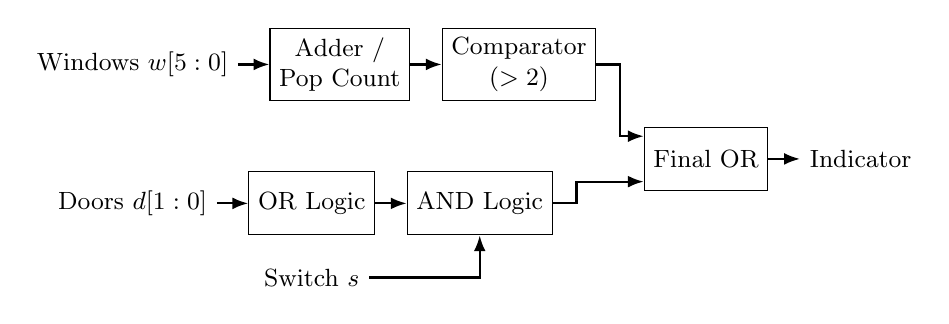
\begin{tikzpicture}[
    box/.style={draw, rectangle, minimum height=0.8cm, minimum width=1.5cm, align=center, font=\small},
    arrow/.style={-{Latex[length=2mm]}, thick}
]

% Nodes
\node (win) {\small Windows $w[5:0]$};
\node [box, right=0.4cm of win] (sum) {Adder / \\ Pop Count};
\node [box, right=0.4cm of sum] (comp) {Comparator \\ ($>2$)};

\node [below=1.2cm of win] (doors) {\small Doors $d[1:0]$};
\node [box, right=0.4cm of doors] (or1) {OR Logic};

\node [below=0.3cm of or1] (switch) {\small Switch $s$};
\node [box, right=0.4cm of or1] (and1) {AND Logic};

\node [box, right=0.6cm of comp, yshift=-1.2cm] (or2) {Final OR};
\node [right=0.4cm of or2] (ind) {\small Indicator};

% Arrows
\draw [arrow] (win) -- (sum);
\draw [arrow] (sum) -- (comp);
\draw [arrow] (comp.east) -- ++(0.3,0) |- (or2.160);

\draw [arrow] (doors) -- (or1);
\draw [arrow] (or1) -- (and1);
\draw [arrow] (switch.east) -| (and1.south);
\draw [arrow] (and1.east) -- ++(0.3,0) |- (or2.200);

\draw [arrow] (or2) -- (ind);

\end{tikzpicture}
}
\end{center}

\section{Problem 2: Sensor Threshold System}

\subsection{Problem Description}
A system reads four 4-bit sensors. A 2-bit address selector dictates which sensor reading is active. If the selected reading is greater than or equal to a user-defined 4-bit threshold, an LED indicator turns on.

\subsection{Solution Architecture}
The design pairs a Multiplexer (MUX) with a Digital Comparator. The 2-bit address selector (\texttt{sel}) drives a 4-to-1 MUX to isolate one of the four 4-bit sensor inputs (\texttt{s0, s1, s2, s3}). The 4-bit output of the MUX is immediately routed into an arithmetic comparator. The comparator evaluates if the MUX output is $\geq$ the 4-bit \texttt{thresh} input, driving the LED high if true.

\vspace{0.5cm}
\begin{center}
\resizebox{\textwidth}{!}{ 
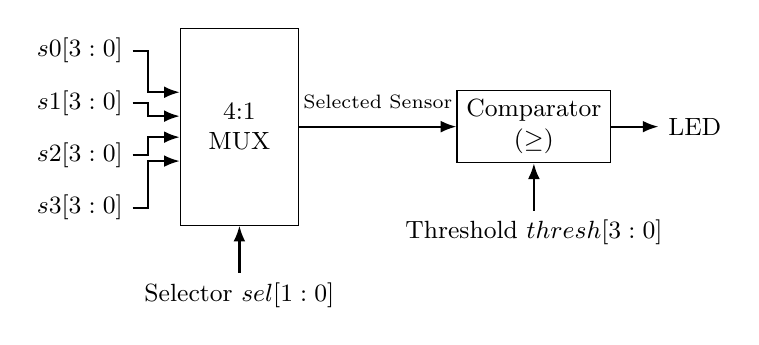
\begin{tikzpicture}[
    box/.style={draw, rectangle, minimum height=0.8cm, minimum width=1.5cm, align=center, font=\small},
    arrow/.style={-{Latex[length=2mm]}, thick}
]

% Nodes
\node (s0) {\small $s0[3:0]$};
\node [below=0.1cm of s0] (s1) {\small $s1[3:0]$};
\node [below=0.1cm of s1] (s2) {\small $s2[3:0]$};
\node [below=0.1cm of s2] (s3) {\small $s3[3:0]$};

\node [box, right=0.6cm of s1, yshift=-0.3cm, minimum height=2.5cm] (mux) {4:1\\MUX};
\node [below=0.6cm of mux] (sel) {\small Selector $sel[1:0]$};

% Increased gap to 1.8cm so the text fits comfortably
\node [box, right=2cm of mux] (comp) {Comparator \\ ($\geq$)};
\node [below=0.6cm of comp] (thresh) {\small Threshold $thresh[3:0]$};

\node [right=0.6cm of comp] (led) {\small LED};

% Arrows
\draw [arrow] (s0.east) -- ++(0.2,0) |- (mux.150);
\draw [arrow] (s1.east) -- ++(0.2,0) |- (mux.170);
\draw [arrow] (s2.east) -- ++(0.2,0) |- (mux.190);
\draw [arrow] (s3.east) -- ++(0.2,0) |- (mux.210);

% Shifted text up slightly with yshift
\draw [arrow] (mux) -- node[above, yshift=0.1cm, font=\scriptsize] {Selected Sensor} (comp);
\draw [arrow] (sel) -- (mux);
\draw [arrow] (thresh) -- (comp);
\draw [arrow] (comp) -- (led);

\end{tikzpicture}
}
\end{center}

\end{document}